\section{Computing Clearance Value Annotations}
\label{aha:planningwithannotations}
A \emph{clearance value} is a distance-to-obstacle metric associated with an octile $t$ and a capability $c$.
It represents the maximal length (or width) of a square whose upper-left octile is $t$ and which contains only octiles whose terrain types are included in $c$.
An octile can have several clearance values associated with it, one for each capability. 
%Note that an octile can have several clearance values associated with it, one for each capability. 
%On a grid map, a clearance value is perhaps best explained as representing the length or width of a square that begins at some octile being evaluated and is expanded symmetrically to the right and down until it intersects an obstacle.     

To make our ideas easier to follow, we will use as a running example a simple environment featuring two terrain types: Ground (represented as white tiles) and Trees (represented as grey tiles). 
To distinguish traversable tiles from non-traversable tiles we will colour hard obstacles black. 
The set of capabilities, $C$, required to traverse such a map is thus defined as $C = \lbrace \lbrace \textit{Ground} \rbrace, \lbrace \textit{Trees} \rbrace, \lbrace \textit{Ground} \vee \textit{Trees} \rbrace \rbrace$. 
We will work with agents of two sizes traversing across this environment and thus let $S = \lbrace 1, 2 \rbrace$.
\par \indent
Figure \ref{aha-fig:annotations} (a) to (d) illustrates how clearance can be computed with an iterative procedure in an environment as described above.
In Figure \ref{aha-fig:annotations}(a) the clearance square for the highlighted traversable target tile is initialised to 1. 
Subsequent iterations (Figures \ref{aha-fig:annotations}(b)-(c)) extend the square and increment the clearance. 
The process continues until the square contains an obstacle (Figure \ref{aha-fig:annotations}(d)) or extends beyond a map boundary at which point we terminate and do not increment clearance any further.
\par \indent
In Figure \ref{aha-fig:annotations}(e) we show the resultant clearance values for the single-terrain $\lbrace \textit{Ground} \rbrace$ capability on a toy map example (note that we omit zero-value clearances).
Similarly, Figure \ref{aha-fig:annotations}(f) and Figure \ref{aha-fig:annotations}(g) show the clearance values associated with the $\lbrace \textit{Trees} \rbrace$ and $\lbrace \textit{Ground} \vee \textit{Trees} \rbrace$ capabilities respectively.  

\begin{figure}[htbp]
	\vspace{-9pt}
       \caption{\emph{(a)-(d) Computing clearance; we expand the square until a hard obstacle is encountered. (e)-(g) Clearance values for different capabilities.} \vspace{0.5em}}
       \begin{center}
                       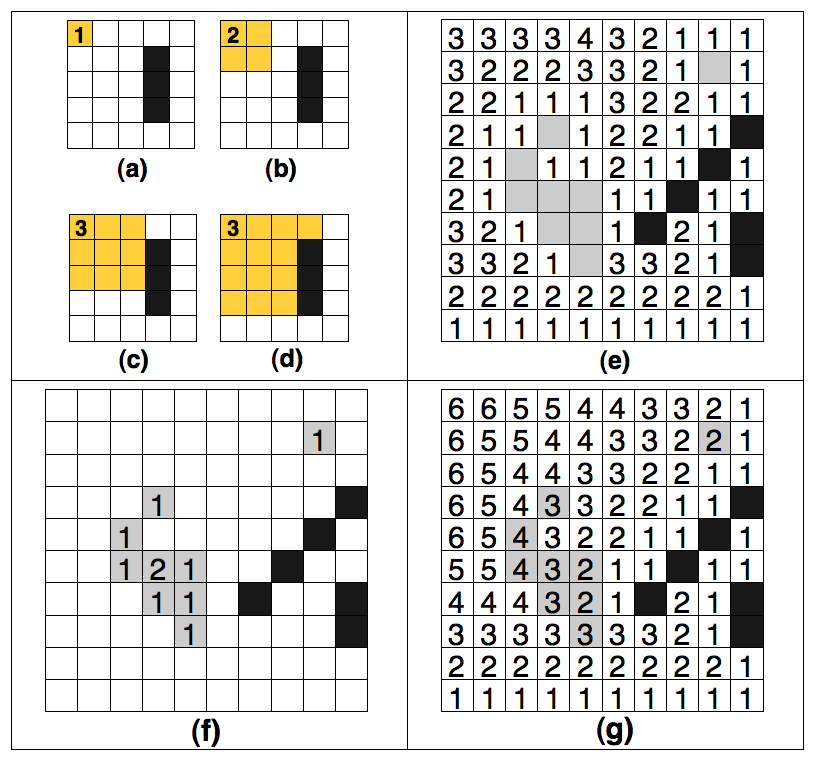
\includegraphics[scale=0.20, trim = 20mm 9mm 20mm 0mm]{diagrams/annotations.png}
       \end{center}
       \label{aha-fig:annotations}
	\vspace{-6pt}
\end{figure}

Once a clearance value is derived we store it in memory and repeat the entire procedure for each capability $c \in C$.  
The algorithm terminates when all octiles $t \in gridmap$ have been considered. 
The worst-case space complexity associated with computing clearance values in this fashion is thus characterised by: 
\begin{lemma}
\label{aha-lemma:numannotations}
Let $CV$ be the set of all clearance values required to annotate an octile gridmap with $r$ terrains. Further, let $G = (V, E)$ be a graph representing the gridmap where $V_{HO} \subseteq V$ is the set of hard obstacles. Then, 
$$|CV| = (|V| - |V_{HO}|)\times 2^{r-1}$$
\end{lemma}

\begin{proof}
For a node to be traversable for some capability, the capability must include the node's terrain type. 
There are $2^{r}$ capabilities but a fixed terrain type is included in only $2^{r-1}$ of these. 
There are $|V|$ nodes in total to represent the environment, and we avoid storing any clearance values for all nodes in $V_{HO}$. 
\end{proof}

The result from Lemma \ref{aha-lemma:numannotations} is an upper bound; if no agent has a given capability $c$ there is no need to store the corresponding clearances.
Despite this observation, the associated exponential growth function suggests that it is impractical to store every clearance value as there are $\Theta(2^{r})$ per node.
Fortunately, clearance values can be computed on-demand with little effort. 
In particular, calculating clearance for any agent $a$ of size $s \in S$ only requires building a clearance square of maximum area $s^2$ octiles. 
We present such an approach in Algorithm \ref{aha-alg:calculateclearance}. 
\input algorithms/alg1_calculateclearance
\par \indent
The key advantage of calculating clearance is that we are able to
%plan for both large and small agents using a fixed size grid. 
%We achieve this by 
map our extended problem into a classical problem, called the \emph{canonical problem}, with only two types of tiles (traversable and blocked) and only atomic-size agents. We formalise this as:
%The next theorem formalizes this result.
\begin{theorem}
\label{aha-theorem:reducibility}
Given an annotated gridmap and an agent of arbitrary size and capability, any path planning problem can be reduced to a classical path planning problem, where the size of the agent is one octile and the capability of the agent is one terrain.
\end{theorem}

\begin{proof}
Consider an agent $a$ of size $s_a$ and capability $c_a$.
Consider further a location $l$ of size $s_a \times s_a$, its upper-left octile $\textit{ul}$,
and the clearance value ${cv}(\textit{ul}, c_a)$ associated with the octile $\textit{ul}$ and the capability $c_a$.
It is easy to observe that the location $l$ is traversable by the agent $a$
if and only if ${cv}(\textit{ul}, c_a) \geq s_a$.
This allows us to map the original problem into a classical path planning problem as follows:
The agent $a$, which currently occupies an $s_a \times s_a$ location $l$, is mapped into an atomic-size agent whose location is $ul$. 
When searching for a path, any octile $t$ is traversable by the atomic-size agent only if ${cv}(t, c_a) \geq s_a$.
All other octiles are regarded as blocked.
%Thus, the agent is able to navigate across a map by only considering the traversal requirements of a single octile.
%Since each tile being evaluated is either traversable or not this is equivalent to solving a single-terrain problem.
\end{proof}
This is a useful result because it indicates that we can apply abstraction techniques from classical path planning to answer much more complex queries involving a wide range of terrain type and agent-size variables. 
%% DH: Do we need to state this? I know it was a problem but we elegantly side-step it via theorem 1. Given that we don't need to solve it (explicitly), do we still need to mention it?
%% if so, would this comment not be better made when we introduce cluster-based abstraction rather than here?
% AB: I think it helps make the claim above stronger.
In particular, if topological abstraction that partitions a gridmap into disjoint clusters were applied directly to a problem with arbitrary-size agents, a large agent could be in several clusters at a time. This raises a number of challenges which we found difficult to handle. The theorem above elegantly eliminates this problem, since an atomic-size agent can be in only one cluster at a time.
